\linespread{1.5}
%use \usepackage{float}
\textbf{Solução}

\textbf{a)}

\begin{figure}[H]
    \centering
    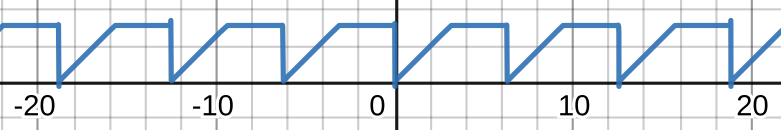
\includegraphics[width = 0.7\linewidth]{fig/sf8a.png}
    \caption{Como foi feita pelo site \textit{https://www.desmos.com/calculator} foi necessário limitar a série, o que permite ver os efeitos causados pela aproximação da série. Além disso no seu desenho deve mostrar os pontos que pertencem ou não aquela parte do gráfico, por exemplo: $x = -2\pi \in y=0$, mas quando $y(2\pi) \neq \pi$, $y$não pertence a , os saltos de uma função pra outra também não existem de fato na função.}
\end{figure}

\textbf{b)}
\begin{equation}
    \label{eq:Fourierserie}
    f(x) = a_0 + \sum_{k=1}^\infty a_k\cos{(kwx)} + b_k\sin{(kwx)}
\end{equation}

Como a série não é par nem ímpar, teremos que calcular todos os coeficientes de Fourier. Temos que nesse caso $T=2\pi \therefore w = \frac{2\pi}{T} = \frac{2\pi}{2\pi} = 1$ 

Comecemos a calcular então:
\begin{equation*}
    a_0 = \frac{1}{T}\int^{T/2}_{-T/2} f(x)dx = \frac{1}{2\pi}\int^\pi_0xdx + \frac{1}{2\pi} \int_\pi^{2\pi}\pi dx
\end{equation*}
\begin{equation*}
    = \frac{1}{2\pi}\left\{\left[\frac{x^2}{2}\right]^\pi_0 + [\pi x]^{2\pi}_\pi\right\} = \frac{1}{2\pi}\left\{\frac{\pi^2}{2} + [2\pi^2 - \pi^2\right\} = \frac{1}{2\pi}\left\{\frac{\pi^2}{2} + \pi^2\right\}
\end{equation*}
\begin{equation}
    \label{eq:sf8ba0}
    \boxed{a_0 = \frac{3\pi^2}{4}}
\end{equation}

Agora $a_n$:
\begin{equation*}
    a_k = \frac{2}{T}\int^{T/2}_{-T/2} f(x)\cos{(kwx)dx} = \frac{1}{\pi}\left\{\int^{\pi}_{0} x\cos{(kwx)dx} + \int^{2\pi}_\pi \pi\cos{(kwx)}dx \right\}
\end{equation*}
\begin{equation}
    \label{eq:sf8banpart}
    a_n=\frac{1}{\pi}\{(I) + (II)\}
\end{equation}

\begin{equation*}
    (I) = \int_0^\pi x\cos{(kwx)} = \left[\frac{x\sin{(kwx)}}{kw}\right]^\pi_0 - \int^{\pi}_0\frac{\sin{(kwx)}}{kx} = \left[\frac{x\sin{(kwx)}}{kw}\right]^\pi_0 + \left[\frac{\cos{(kwx)}}{(kw)^2}\right]^\pi_0
\end{equation*}
\begin{equation*}
    \left[\frac{\pi\sin{k\pi}}{k} - 0 \right] + \left[\frac{k\pi}{k^2} - \frac{\cos0}{k^2}\right]
\end{equation*}

Como temos que $\sin{(k\pi) } = 0\forall k \in \Z$, assim como $\cos{(k\pi)} = (-1)^k$, temos então que:
\begin{equation}
    \label{eq:sf8banI}
    (I) = \frac{(-1)^k - 1}{k^2}
\end{equation}

\begin{equation}
    \label{eq:sf8banII}
    (II) = \int_\pi^{2\pi} \pi\cos{(kwx)}dx = \left[\frac{\pi\sin{(kwx)}}{kw}\right]^{2\pi}_\pi = 0
\end{equation}
isso pela mesma razão comentada acima sobre o $\sin{(k\pi)}$.

Assim, substituindo \ref{eq:sf8banI} e \ref{eq:sf8banII} em \ref{eq:sf8banpart}, obtemos que:
\begin{equation}
    \label{eq:sf8ban}
    a_k = \frac{(-1)^k - 1}{\pi k^2} \xrightarrow{} \boxed{a_k = \frac{(-1)^{2k-1} - 1}{\pi (2k-1)^2}}
\end{equation}
Esse último passo se deve ao fato que pra todo $k$ par, $a_n = 0$, logo apresentamos somente para aqueles resultados não nulos. 
Por fim $b_k$:
\begin{equation*}
    b_k = \frac{2}{T}\int^{T/2}_{-T/2} f(x)\sin{(kwx)dx} = \frac{1}{\pi}\left\{\int^\pi_0 x\sin{(kwx)}dx + \int_\pi^{2\pi} \pi \sin{(kwx)}dx\right\}
\end{equation*}
\begin{equation}
    \label{eq:sf8bbks}
    b_k = \frac{1}{\pi}\{(III) + (IV)\}
\end{equation}
Resolvendo $(III)$:
\begin{equation*}
    (III) = \int^\pi_0 x\sin{(kwx)}dx = \left[\frac{-x\cos{(kwx)}}{kw}\right]^\pi_0 - \int^\pi_0 \frac{-\cos{(kwx)}}{kw}dx
\end{equation*}
Desta, se sabe que a integral que aparece quando se resolve por partes resulta em $0$, e substituindo $w$, teremos:
\begin{equation*}
    (III) = \frac{-\pi\cos{(kwx)}}{k}
\end{equation*}
daqui sabemos que $\cos{(kwx)} = (-1)^k$
\begin{equation}
   \label{eq:sf8bbn3}
   (III) = \frac{-\pi(-1)^k}{k}
\end{equation}

Agora resolvemos $(IV)$:
\begin{equation*}
    (IV) = \int_\pi^{2\pi} \pi \sin{(kwx)}dx = \left[\frac{-\pi\cos{(kwx)}}{kw}\right]^{2\pi}_\pi =^{w=1} \frac{-\pi\cos{(2\pin)}}{k} + \frac{\pi\cos{(k\pi)}}{k}
\end{equation*}
\begin{equation}
    \label{eq:sf8bbn4}
    (IV) = \frac{\pi(-1)^k - \pi}{k}
\end{equation}

Agora se substituirmos \ref{eq:sf8bbn3} e \ref{eq:sf8bbn4} em \ref{eq:sf8bbks} obtemos que:
\begin{equation}
    \label{eq:sf8bbk}
    b_k = \frac{1}{\pi}\left(\frac{-\pi(-1)^k}{k} + \frac{\pi(-1)^k}{k} + \frac{-\pi}{k}\right) \xrightarrow{} \boxed{b_k = \frac{-1}{k}}
\end{equation}

E por fim substituímos \ref{eq:sf8ba0}, \ref{eq:sf8ban} e \ref{eq:sf8bbk} em \ref{eq:Fourierserie}, obtemos por fim:

\begin{equation}
    \boxed{f(x) = \frac{3\pi}{4} + \sum^\infty_{k=1} \frac{(-1)^{2k-1} - 1}{\pi (2k-1)^2} \cos{[(2k-1)x]} - \frac{1}{k}\sin{(kx)} 
    }
\end{equation}